\documentclass[../main/main.tex]{subfiles}

\raggedbottom

\makeatletter
\renewcommand{\@chapapp}{Optique -- chapitre}
\makeatother

\begin{document}
\setcounter{chapter}{1}

\chapter{Base de l'optique g\'eom\'etrique}

\section{Propriétés générales}

\subsection{Approximation de l'optique géométrique}

\begin{defi}[label=def:optgeo, hand]{approximation de l'optique géométrique}

    L'approximation de l'optique géométrique consiste à négliger tout phénomène
    de diffraction (et d'interférence, cf.\ chapitres plus avancés) pour ignorer
    le comportement ondulatoire de la lumière. Dans cette approche, la lumière
    est équivalente à un flux de particules \textit{indépendantes}, sans
    interaction globale (propriété d'une onde)~: c'est le modèle corpusculaire.

\end{defi}

\subsection{Notion de rayon lumineux}

Dans le cadre de l'optique géométrique, on décrit donc la lumière par la
trajectoire des photons.

\begin{tcbraster}[raster columns=3, raster equal height=rows]
    \begin{defi}[label=def:rl, raster multicolumn=2]{rayon et faisceau lumineux}

        On appelle «~rayon lumineux~» le chemin que semble suivre la lumière
        entre deux points lors d'une expérience de propagation. C'est une
        \textbf{courbe orientée} donnant la direction et le sens de propagation
        d'une onde lumineuse.\bigbreak

        On appelle «~faisceau lumineux~» passant
        par un point l'ensemble des rayons lumineux passant par ce point.

    \end{defi}
    \begin{NCrema}[]{Remarque}

        C'est un outil théorique~: il est impossible d'isoler un rayon lumineux
        en pratique à cause de la diffraction.

    \end{NCrema}
\end{tcbraster}

\subsection{Propagation rectiligne}

\begin{tcbraster}[raster columns=2, raster equal height=rows]
    \begin{prop}[label=prop:prop_rect, valign=center]{propagation rectiligne}

        \bfseries Dans un milieu TLHI, la lumière se propage en ligne droite.

    \end{prop}
    \begin{NCcexe}[]{Contre-exemple}

        L'indice optique changeant avec la température, dans certaines
        conditions l'atmosphère n'est pas homogène~: cela peut causer des
        mirages (trajectoire courbée de la lumière).

    \end{NCcexe}
\end{tcbraster}

\subsection{Retour inverse de la lumière}

\begin{tcbraster}[raster columns=2, raster equal height=rows]
    \begin{prop}[label=prop:ret_inv]{retour inverse}
        Dans un milieu TLI, homogène ou non, le trajet suivi par la lumière
        entre deux points situés sur un même rayon lumineux est indépendant du
        sens de propagation.
    \end{prop}
    \begin{impl}[label=impl:ret_inv]{échange}
        Si on connaît le trajet dans un sens, on le connaît l'autre sens. On
        utilisera ce raisonnement à plusieurs reprises pour l'étude des systèmes
        optiques.
    \end{impl}
\end{tcbraster}

\subsection{Indépendance des rayons lumineux}

\begin{prop}[label=prop:ind_lum]{indépendance des rayons lumineux}
    Les rayons lumineux n'interfèrent pas entre eux. Notamment, un rayon ne peut
    pas en dévier un autre.
\end{prop}

\section{Lois de Snell-Descartes}

\subsection{Changement de milieu}

\begin{tcbraster}[raster columns=2, raster equal height=rows]
    \begin{tcolorbox}[blankest, raster multicolumn=1, space to=\myspace]
        \begin{tcbraster}[raster columns=1]
            \begin{defi}[label=def:dioptre, add to natural height=\myspace,
                valign=center]{dioptre}

                On appelle «~dioptre~» la surface de séparation entre deux
                milieux transparents d'indices optiques différents.

                \tcblower
                \vfill
                \begin{center}
                    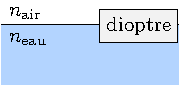
\includegraphics[width=.8\linewidth]{dioptre.pdf}
                    \captionof{figure}{Exemple de dioptre.}
                    \label{fig:dioptre}
                \end{center}
            \end{defi}
            \begin{nota}[label=nota:descartes]{vocabulaire général}
                \begin{itemize}

                    \item On appelle \textbf{point d'incidence} $I$ le point
                        d'intersection entre le rayon incident et le dioptre~;
                    \item On appelle \textbf{plan d'incidence} le plan contenant
                        le rayon incident et la normale au dioptre en I~;
                    \item On appelle \textbf{angle d'incidence} $i_1$ l'angle
                        entre la normale et le rayon incident~;
                    \item On appelle \textbf{angle de réflexion} $r$ l'angle
                        entre la normale et le rayon réfléchi~;
                    \item On appelle \textbf{angle de réfraction} $i_2$ l'angle
                        entre la normale et le rayon réfracté.

                \end{itemize}
            \end{nota}
        \end{tcbraster}
    \end{tcolorbox}
    \begin{tcolorbox}[blankest, raster multicolumn=1]
        \begin{tcbraster}[raster columns=1]
            \begin{prop}[label=prop:r_dioptre]{{réflexion, réfraction}}

                Au niveau d'un dioptre, un rayon lumineux incident donne
                naissance à un rayon réfracté (traversant le dioptre) et à un
                rayon réfléchi.

                \tcblower

                \begin{center}
                    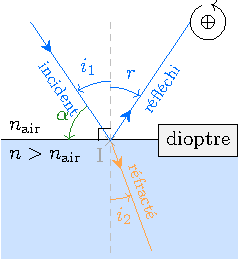
\includegraphics[width=.8\linewidth]{dioptre_rl.pdf}

                    \captionof{figure}{Rayons incidents, réfléchis et réfractés
                    sur un dioptre.}

                    \label{fig:dioptre_rl}
                \end{center}

            \end{prop}
            \begin{ror}[label=ror:normale, valign=center]{calcul des angles}

                \Huge Les angles se calculent entre le rayon et la
                \textbf{normale} au dioptre. Le sens de comptage doit être
                indiqué sur la figure.

            \end{ror}
        \end{tcbraster}
    \end{tcolorbox}
\end{tcbraster}

\subsection{Lois de Snell-Descartes}

\begin{loi}[label=loi:snelldescartes]{Lois de Snell-Descartes}
    Les rayons réfléchi et réfracté appartiennent au plan d'incidence,
    et respectent
    \begin{equation*}
        \boxed{r = -i_1}
        \quad\text{et}\quad
        \boxed{n_1\sin(i_1) = n_2\sin(i_2)}
    \end{equation*}
    \tcblower
    \begin{minipage}{0.45\linewidth}
        \begin{center}
            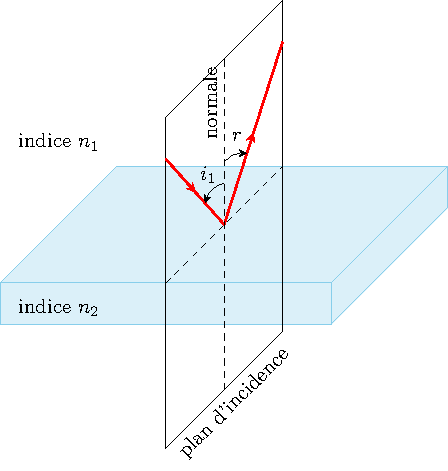
\includegraphics[width=\linewidth]{snell_refl.pdf}
            \captionof{figure}{Réflexion d'un rayon incident}
            \label{fig:snell_refl}
        \end{center}
    \end{minipage}
    \hfill
    \begin{minipage}{0.45\linewidth}
        \begin{center}
            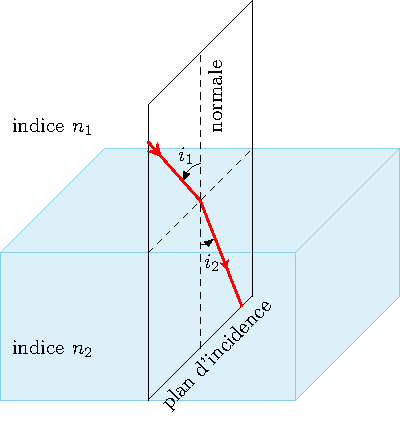
\includegraphics[width=\linewidth]{snell_refr_nsup.pdf}
            \captionof{figure}{Réfraction d'un rayon incident avec $n_2 > n_1$.}
            \label{fig:snell_refl}
        \end{center}
    \end{minipage}
\end{loi}

\begin{impl}[label=impl:refr]{réfraction}
    On distingue 3 cas généraux pour la réfraction~:
    \begin{enumerate}

        \item Si $i_1 = 0$, alors $i_2 = 0$~: en incidence dite «~normale~», il
            n'y a pas de déviation du rayon~;
        \item Si $n_2 > n_1$\footnote{On dit alors que le milieu 2 est
            \textit{plus réfringent} que le milieu 1.}, alors $ \left| i_2
            \right| < \left| i_1 \right|$~: le rayon réfracté se rapproche de la
            normale~;
        \item Si $n_2 < n_1$\footnote{On dit alors que le milieu 2 est
            \textit{moins réfringent} que le milieu 1.}, alors $|i_2| > |i_1|$~:
            le rayon réfracté s'écarte de la normale.

    \end{enumerate}
    Par le principe du retour inverse de la lumière (\ref{prop:ret_inv}), le
    troisième point se déduit du deuxième.
\end{impl}

\newpage

\subsection{Phénomène de réflexion totale}

À partir du moment où $n_2 > n_1$, le rayon réfracté se rapproche toujours de la
normale, et existera toujours. En revanche, si $n_2 < n_1$, le rayon réfracté
s'écarte de la normale. On considère qu'il existe uniquement s'il reste à
l'intérieur du milieu $n_2$, soit par définition $|i_2| <
\frac{\pi}{2}\si{rad}$.

\begin{tcbraster}[raster columns=3, raster equal height=rows]
    \begin{prop}[label=prop:ilim, valign=center]{angle limite de réflexion
        totale}
        Lors du passage d'un milieu plus réfringent à un milieu moins réfringent
        ($n_2 < n_1$), il existe un angle incident limite $i_{\rm lim}$ au-delà
        duquel il n'y a pas de rayon réfracté~: on parle de \textbf{réflexion
        totale}. On a
        \[ \boxed{|i_{\rm lim}| = \arcsin \left( \frac{n_2}{n_1} \right)}\]
    \end{prop}
    \begin{demo}[label=demo:ilim, raster multicolumn=2]{angle limite de
        réflexion totale}
        Soit $i_{\rm lim}$ l'angle d'incidence limite de réfraction, tel que
        $i_2 = \frac{\pi}{2}$. On a~:
        \begin{equation*}
            i_2 = \frac{\pi}{2} \Rightarrow \sin(i_2) = 1
        \end{equation*}
        Or, $n_2\sin(i_2) = n_1\sin(i_{\rm lim})$ d'après la loi de
        Snell-Descartes pour la réfraction. Ainsi,
        \begin{align*}
            n_2 \underbrace{\cancel{\sin(i_2)}}_{=1} & = n_1\sin(i_{\rm lim})\\
            \Leftrightarrow \frac{n_2}{n_1} & = \sin(i_{\rm lim})\\
            \Rightarrow i_{\rm lim} & = \arcsin \left( \frac{n_2}{n_1} \right)
        \end{align*}
    \end{demo}
\end{tcbraster}

\begin{exem}[label=exem:ilim]{réflexion totale}
    \begin{center}
        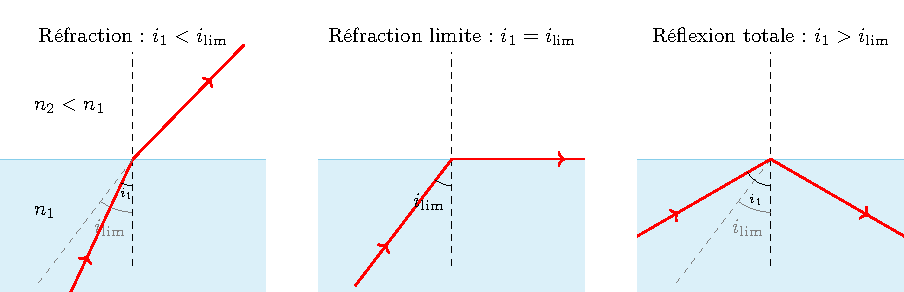
\includegraphics[width=\linewidth]{snell_refl_tot.pdf}
        \captionsetup{justification=centering}
        \captionof{figure}{Phénomène de réflexion totale}
        \label{fig:refl_tot}
    \end{center}
\end{exem}

\section{Généralités sur les systèmes optiques}
\subsection{Définition}

\begin{tcbraster}[raster columns=2, raster equal height=rows]
    
    \begin{defi}[label=def:so]{Système optique}
    
        On appelle système optique un ensemble de composants optiques (dioptres,
        miroirs) rencontrés successivement par les rayons lumineux.
    
    \end{defi}
    \begin{NCexem}[]{Exemple}
        L'exemple le plus simple est le miroir plan.
    \end{NCexem}
\end{tcbraster}

\subsection{Système centré}
\begin{tcbraster}[raster columns=2, raster equal height=rows]
    \begin{defi}[label=def:vocso]{Systèmes centrés}

        On appelle système \textit{centré} un système optique invariant par
        rotation autour d'un axe~; cet axe est alors appelé \textit{axe
        optique}. \textbf{On l'oriente dans le sens de propagation de la lumière
        incidente}, et les distances sont considérées algébriquement (affectées
        d'un signe). On notera par exemple $\obar{AB} = \SI{-2}{cm}$.

    \end{defi}
    \begin{NCexem}[width=\linewidth]{Schéma}
        \begin{center}
            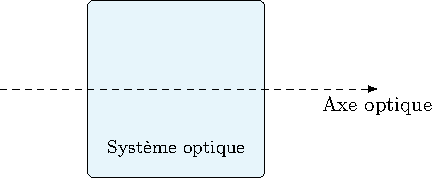
\includegraphics[width=\linewidth]{syst_opt.pdf}
            \captionof{figure}{Système optique centré.}
            \label{fig:socent}
        \end{center}
    \end{NCexem}
\end{tcbraster}

\subsection{Rayons incidents, rayons émergents}

\begin{tcbraster}[raster columns=2, raster equal height=rows]
    
    \begin{defi}[label=def:rlie]{Rayons incidents et émergents}
    
        On appelle \textbf{rayons incidents} les rayons entrant par la face
        d'entrée d'un système optique. On appelle \textbf{rayons émergents} les
        rayons sortant par la face de sortie d'un système optique.
    
    \end{defi}
    \begin{NCexem}[width=\linewidth]{Schéma}
        \begin{center}
            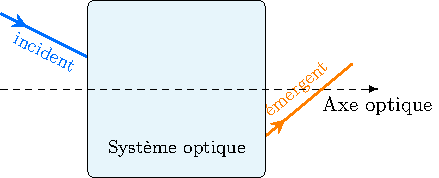
\includegraphics[width=\linewidth]{syst_opt_ie.pdf}
            \captionof{figure}{Rayons incidents, émergents.}
            \label{fig:socent}
        \end{center}
    \end{NCexem}
\end{tcbraster}

\subsection{Faisceaux lumineux}

\begin{tcbraster}[raster columns=4, raster equal height=rows]
    \begin{defi}[label=def:faisceau]{Faisceaux lumineux}
        On appelle \textit{faisceau lumineux} un ensemble de rayons lumineux. Un
        faisceau peut être \textit{convergent}, \textit{divergent} ou
        \textit{parallèle}.
    \end{defi}    
    \begin{NCexem}[raster multicolumn=3]{Schéma}
        \begin{center}
            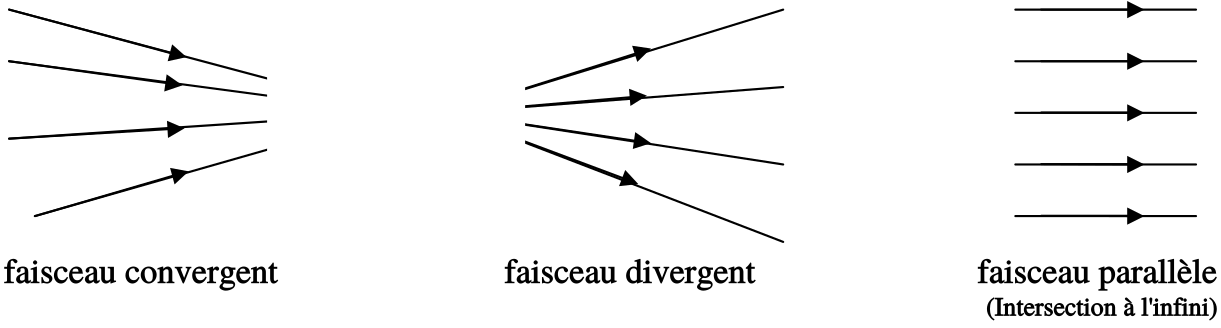
\includegraphics[width=\linewidth]{ch2_fig8.png}
            \captionof{figure}{Natures de faisceaux}
            \label{fig:faisceau}
        \end{center}
    \end{NCexem}
\end{tcbraster}

\subsection{Objets et images réelles ou virtuelles}

\begin{defi}[label=def:objimg, sidebyside]{Objet et image}
    On appelle point \textbf{objet} d'un système optique le point d'intersection
    des rayons \textbf{incidents}.
    \tcblower
    On appelle point \textbf{image} d'un système optique le point d'intersection
    des rayons \textbf{émergents}.
\end{defi}

\begin{defi}[label=reelvirt, sidebyside]{Réel et virtuel}
    Un point objet est \textbf{réel} si le faisceau \textbf{incident} est
    \textbf{divergent}. Il est \textbf{virtuel} si le faisceau est
    \textbf{convergent}.
    \tcblower
    Un point image est \textbf{réel} si le faisceau \textbf{émergent} est
    \textbf{convergent}. Il est \textbf{virtuel} si le faisceau est
    \textbf{divergent}.
\end{defi}

On trouve aussi les définitions suivantes, plus communément admises (mais plus
verbeuses).

\begin{defi}[label=reelvirt2, sidebyside]{{Réel et virtuel, bis}}
    Un point \textbf{objet} est \textbf{réel} s'il est placé \textbf{avant la
    face d'entrée} du système, et \textbf{virtuel sinon}.
    \tcblower
    Un point \textbf{image} est \textbf{réel} s'il est placé \textbf{après la
    face de sortie} du système, et \textbf{virtuel sinon}.
\end{defi}

\begin{exem}[label=exem:rellvirt]{Objets et images réelles}
    \begin{minipage}{0.45\linewidth}
        \begin{center}
            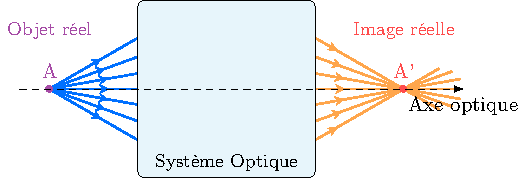
\includegraphics[width=\linewidth]{obj_r-img_r.pdf}
            \captionof{figure}{Objet et image réelles.}
            \label{fig:objrimgr}
        \end{center}
    \end{minipage}
    \hfill
    \begin{minipage}{0.45\linewidth}
        \begin{center}
            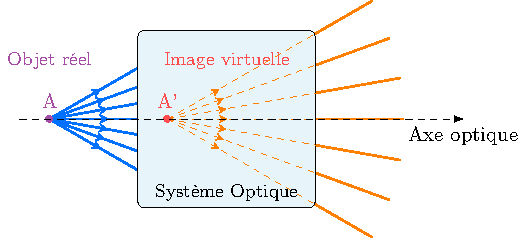
\includegraphics[width=\linewidth]{obj_r-img_v.pdf}
            \captionof{figure}{Objet réel et image virtuelle.}
            \label{fig:objrimgv}
        \end{center}
    \end{minipage}
    \begin{minipage}{0.45\linewidth}
        \begin{center}
            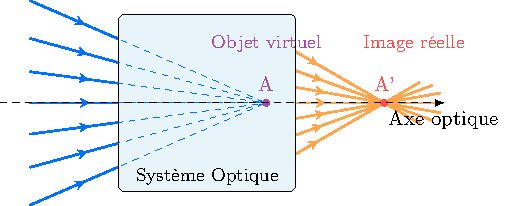
\includegraphics[width=\linewidth]{obj_v-img_r.pdf}
            \captionof{figure}{Objet virtuel et image réelle.}
            \label{fig:objvimgr}
        \end{center}
    \end{minipage}
    \hfill
    \begin{minipage}{0.45\linewidth}
        \begin{center}
            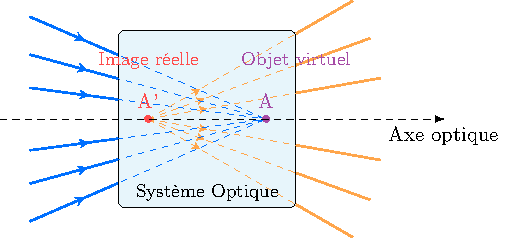
\includegraphics[width=\linewidth]{obj_v-img_v.pdf}
            \captionof{figure}{Objet et image virtuelles.}
            \label{fig:objvimgv}
        \end{center}
    \end{minipage}
\end{exem}

\begin{impl}[label=impl:objimg_espace,
             sidebyside, righthand width=.7\textwidth]{Espaces objet et image}
    De par ces définitions, on peut définir les zones spatiales d'un système
    optique dans lesquelles un objet ou une image sera soit réel, soit virtuel.
    \tcblower
    \begin{center}
        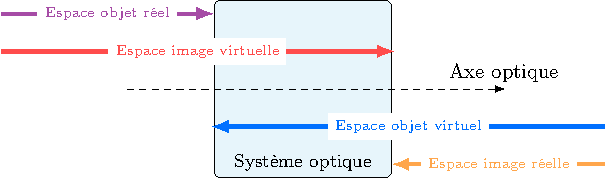
\includegraphics[width=\linewidth]{objimg_espace.pdf}
        \captionof{figure}{Espaces objet et image.}
        \label{fig:objimg_espace}
    \end{center}
\end{impl}

\begin{nota}[label=nota_opt]{conjugaison de 2 points}
    Lorsqu'un point objet $A$ passe par un système optique $S$ pour former
    l'image $A'$, on dit que $A$ et $A'$ sont \textit{conjugués par le système}.
    Schématiquement, on note cette relation
    \[\boxed{A\opto{S}{}A'}\]
    Dans cette notation, $A$ est un objet \textbf{pour $S$}, et $A'$ est une
    image \textbf{pour $S$}. Nous serons amené-es à étudier des combinaisons de
    systèmes optiques dans lesquels un point sera à la fois image de l'un et
    objet du suivant.
\end{nota}

\subsection{Objet étendu, grandissement transversal}
\begin{tcbraster}[raster columns=3, raster equal height=rows]
    \begin{defi}[label=def:objet]{objet étendu et angle apparent}
    
        On appelle \textit{objet étendu} un ensemble de points objets continu,
        considéré comme une infinité de points objets.\bigbreak

        L'\textit{angle apparent} d'un objet étendu est l'angle perçu (par un
        détecteur~: œil, caméra…) entre les rayons émis par les extrémités de
        l'objet.
    
    \end{defi}
    \begin{defi}[label=def:grand, raster multicolumn=2,
        sidebyside]{grandissement transversal}

        Soit $\obar{AB}$ un objet étendu avec $A$ sur l'axe optique, passant par
        un système $S$ donnant une image elle aussi étendue $\obar{A'B'}$. On
        appelle \textit{grandissement transversal} et on le note $\gamma$ le
        rapport

        \[\boxed{\gamma = \frac{\ABb}{\ABp}}\]
        pour $AB \opto{S}{} A'B' $
        \tcblower
        \begin{center}
            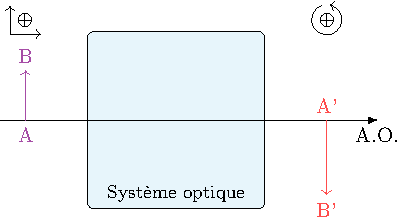
\includegraphics[width=\linewidth]{syst_opt_objet.pdf}
            \captionof{figure}{Objet et image étendues.}
            \label{fig:obj_et}
        \end{center}
    \end{defi}
\end{tcbraster}

\subsection{Foyers d'un système optique}

\begin{defi}[label=def:foy, sidebyside]{Foyers principaux image et objet}

    Le foyer principal objet $F$ est le \textbf{point objet} d'un système
    donnant une \textbf{image à l'infini} (rayons parallèles entre eux) avec des
    rayons parallèles à l'axe optique. Le plan perpendiculaire à l'axe optique
    et passant par $F$ est appelé \textit{plan focal objet}. On note

    \[\boxed{F \opto{S}{} \underset{\text{sur l'axe optique}}{\infty}}\]
    \begin{center}
        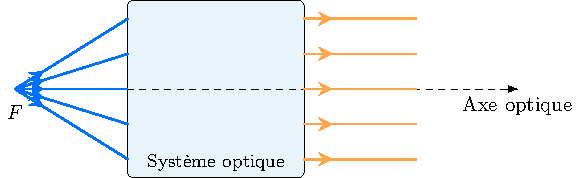
\includegraphics[width=\linewidth]{fobj.pdf}
        \captionof{figure}{Foyer principal objet.}
        \label{fig:fobj}
    \end{center}
    
    \tcblower

    Le foyer principal image $F'$ est le \textbf{point image} d'un système d'un
    \textbf{objet situé à l'infini} (rayons parallèles entre eux) avec des
    rayons parallèles à l'axe optique. Le plan perpendiculaire à l'axe optique
    et passant par $F'$ est appelé \textit{plan focal image}. On note

    \[\boxed{\underset{\text{sur l'axe optique}}{-\infty} \opto{S}{} F'}\]
    \begin{center}
        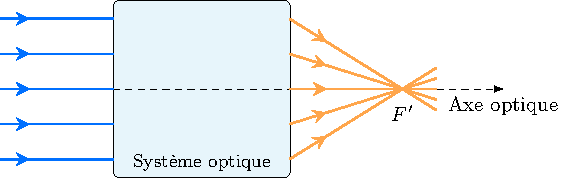
\includegraphics[width=\linewidth]{fimg.pdf}
        \captionof{figure}{Foyer principal image.}
        \label{fig:fimg}
    \end{center}
    
\end{defi}

\begin{tcbraster}[raster columns=3, raster equal height=rows]
    \begin{rema}[label=rema:retinv]{retour inverse}
    
        Nous pouvons en quelque sorte déduire le fonctionnement du système
        optique dans le second cas en utilisant le principe du \textbf{retour
        inverse de la lumière}, en «~remontant le film~».
    
    \end{rema}
    \begin{prop}[label=prop:foy]{foyers principaux}
    
        En plus d'être une définition, c'est une propriété~: \textbf{tous rayons
            incidents qui se croisent en $F$ émergent parallèles à l'axe
            optique, et tous rayons incidents parallèles à l'axe optique
        émergent en se croisant en $F'$}.
    
    \end{prop}
    \begin{coro}[label=coro:foysec]{foyers secondaires}
    
        Tous rayons incidents \textbf{parallèles entre eux} émergent en se
        \textbf{croisant dans le plan focal image}\footnote{en un point appelé
        \textit{foyer secondaire image} $\Phi'$}, et tous rayons incidents se
        \textbf{croisant dans le plan focal objet}\footnote{en un point appelé
        \textit{foyer secondaire objet} $\Phi$} émergent \textbf{parallèles
    entre eux}.
    
    \end{coro}
\end{tcbraster}

\section{Approximation de Gauss}

\subsection{Stigmatisme, aplanétisme}

\begin{tcbraster}[raster columns=2, raster equal height=rows]
    \begin{defi}[label=def:stig]{stigmatisme}

        Un système optique est dit \textit{stigmatique} si tous les rayons émis
        par un point objet $A$ convergent en un seul point image $A'$. Il ne
        l'est pas si l'image d'un point forme une tâche.

    \end{defi}
    \begin{defi}[label=def:apla]{aplanétisme}

        Un système optique est dit \textit{aplanétique} si un objet étendu
        $\obar{AB}$ perpendiculaire à l'axe optique donne une image
        $\obar{A'B'}$ également perpendiculaire à l'axe optique.

    \end{defi}
\end{tcbraster}

\subsection{Rigoureux ou approché ?}

La plupart des systèmes optiques (lentilles, œil, appareil photo…) ne sont pas
rigoureusement stigmatiques et aplanétiques~: il arrive souvent qu'un point
source forme une tâche sur un capteur (astigmatisme) ou qu'une droite soit vue
courbée (non-aplanétisme). On peut cependant trouver des conditions
dans lesquelles le stigmatisme et l'aplanétisme sont approchés, par exemple si
la tâche formée par le système est plus petite que l'élément récepteur (pixel
pour une caméra).

\subsection{Conditions de Gauss}

\begin{tcbraster}[raster columns=2, raster equal height=rows]
    
    \begin{defi}[label=def:gausscond]{Rayons paraxiaux}

        Un système optique est utilisé dans les conditions de Gauss lorsqu'il
        est éclairé par des rayons \textbf{paraxiaux}, c'est-à-dire

        \begin{enumerate}
            \item peu éloignés de l'axe optique~;
            \item peu inclinés par rapport à l'axe optique.
        \end{enumerate}
    \end{defi}
    \begin{prop}[label=prop:gaussprop]{approximation de Gauss}
    
        Dans les conditions de Gauss, un système centré respecte les conditions
        de stigmatisme et d'aplanétisme \textit{approchés}. On les
        \textbf{considérera} comme rigoureux tant dans les tracés que dans les
        calculs.
    
    \end{prop}
\end{tcbraster}

%\theendnotes

\end{document}
